\documentclass[First Project.tex]{subfiles}
\begin{document}

\subsection{\textlatin{\textbf{PA = LU}} αποσύνθεση}

Η μέθοδος της \textlatin{\textbf{PA = LU}} αποσύνθεσης στηρίζεται στην μέθοδο του \textlatin{\textbf{Gauss}}, την οποία βελτιώνει έτσι ώστε να αποφευχθούν 
σφάλματα αλλά και για να μπορούν να επιλυθούν πολλά συστήματα της μορφής \textlatin{\textbf{Ax = b}} με τον ίδιο πίνακα \textlatin{\textbf{A}} των 
συντελεστών των αγνώστων και διαφορετικό πίνακα στήλη \textlatin{\textbf{b}} των αγνώστων. Η συνάρτηση που έχει υλοποιηθεί στο αρχείο 
\textlatin{\textbf{lu\_decomposition.py}} υλοποιεί τον παρακάτω αλγόριθμο :
\begin{itemize}
    \item Για κάθε γραμμή του πίνακα $Α$ βρες το απολύτως μεγαλύτερο στοιχείο που πρέπει να μπει στην κύρια διαγώνιο ως \textlatin{pivot}.
    \item Αντιμετάθεσε αν απαιτείται την τωρινή γραμμή με την γραμμή που περιέχει το \textlatin{pivot} στους πίνακες \textlatin{U,P} και \textlatin{L}.
    \item Κάνε απαλοιφή \textlatin{Gauss}.
    \item Όταν οι γραμμές του πίνακα $Α$ τελειώσουν λύσε το σύστημα $Lc = Pb$ ως προς $c$.
    \item Έπειτα λύσε το σύστημα $Ux = c$ ως προς $x$.
    \item Η λύση του συστήματος είναι το παραπάνω διάνυσμα $x$.
\end{itemize}

Πιο συγκεκριμένα, η συνάρτηση \textlatin{\textbf{lu}} δέχεται ως παραμέτρους τον πίνακα \textlatin{A} και το διάνυσμα \textlatin{b} και
επιστρέφει την λύση του συστήματος $x$. Αρχικά, η συνάρτηση πραγματοποιεί τις κατάλληλες αρχικοποιήσεις των πινάκων $P$,$L$ και $U$. Ο πίνακας
$U$ στην αρχή είναι ίδιος με τον $A$ έτσι ώστε η συνάρτηση να μην πραγματοποιήσει καμία αλλαγή στον $A$. Στην συνέχεια, για κάθε γραμμή του 
πίνακα $U$ η συνάρτηση βρίσκει το απολύτως μεγαλύτερο στοιχείο και το μεταφέρει στην κύρια διαγώνιο, οι αλλαγές γραμμών γίνονται παράλληλα στους
πίνακες $P$,$L$ και $U$. Μετά την εύρεση του μεγαλύτερου στοιχείου η συνάρτηση εκτελεί την κλασσική απαλοιφή \textlatin{\textbf{Gauss}} και
συνέχιζει την παραπάνω διαδικάσια για όλες τις γραμμές του πίνακα $U$. Έπειτα, στην κύρια διαγώνιο του $L$ τοποθετούνται 1 και η συνάρτηση 
συνεχίζει με την επίλυση του συστήματος $Lc = Pb$ από πάνω προς τα κάτω ως προς $c$. Τέλος, η συνάρτηση επιλύει το σύστημα $Ux = c$ από κάτω
προς τα πάνω ως προς $x$ όπου τελικά υπολογίζεται η λύση $x$ του συστήματος $Ax = b$ και επιστρέφεται στην καλούσα συνάρτηση. Τονίζεται ότι
η διαδικάσια της \textlatin{\textbf{PA = LU}} αποσύνθεσης στα βήματα πριν την επίλυση του συστήματος $Lc = Pb$ δεν εξαρτάται από το διάνυσμα 
\textlatin{\textbf{b}} και επομένως αν για κάποια προβλήματα ο πίνακας των συντελεστών \textlatin{\textbf{A}} είναι ίδιος αλλά αλλάζει το 
διάνυσμα \textlatin{\textbf{b}} μπορεί να πραγματοποιηθεί \textbf{μία} φορά η \textlatin{\textbf{PA = LU}} αποσύνθεση και στην συνέχεια να
λυθούν τα συστήματα για τα αντίστοιχα \textlatin{\textbf{b}}. Έτσι, το κόστος είναι μία φορά της τάξης του $n^{3}$ για την διαδικάσια
\textlatin{\textbf{PA = LU}} και στην συνέχεια $n^{2}$ για κάθε διαφορετικό \textlatin{\textbf{b}}. Στην συνέχεια, παρουσιάζεται ένα παράδειγμα
επίλυσης ενός γραμμικού συστήματος με την χρήση της συνάρτησης \textlatin{\textbf{lu}} με το οποίο τελειώνει αυτή η παράγραφος. Το σύστημα είναι
το παρακάτω 
\begin{gather*}
    3x_{1} + x_{2} - 4x_{3} + x_{4} = 1 \\
    -5x_{1} + 2x_{2} + x_{3} - 2x_{4} = -3 \\
    -x_{1} + 6x_{2} - 3x_{3} - 4x_{4} = 2 \\
    -2x_{1} + x_{2} - 4x_{3} + 2x_{4} = 0
\end{gather*}
Για την λύση του παραπάνω συστήματος αρχικά δημιουργούμε τον πίνακα $A$ και το διάνυσμα $b$. Στην συνέχεια καλούμε την συνάρτηση 
\textlatin{\textbf{lu}} με ορίσματα τον πίνακα $Α$ και το διάνυσμα $b$ από την οποία παίρνουμε τα παρακάτω αποτελέσματα
\begin{figure}[h!]
    \centering
    \captionsetup{justification=centering}
    \begin{center}
        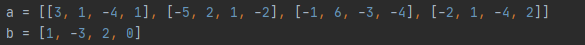
\includegraphics[scale=0.7]{exercise_3_pa_lu_matrices.png}    
        \caption{ Δημιουργία πινάκων για το παραπάνω σύστημα }
    \end{center}
\end{figure} 
\begin{figure}[h!]
    \centering
    \captionsetup{justification=centering}
    \begin{center}
        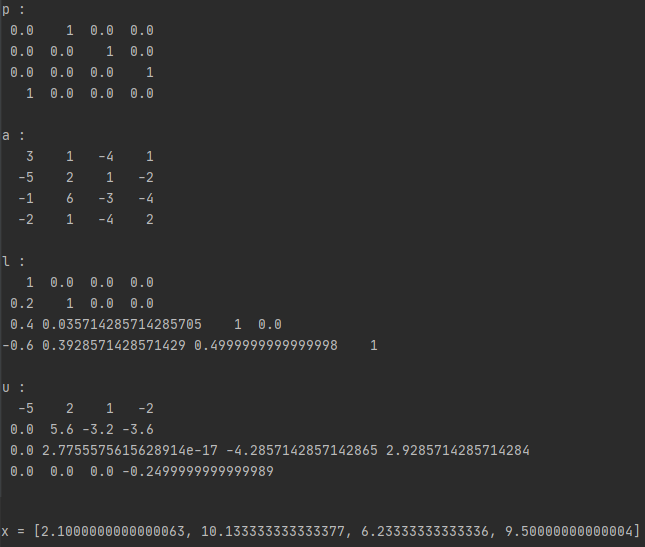
\includegraphics[scale=0.5]{exercise_3_solution.png}    
        \caption{ \textlatin{\textbf{ PA = LU}} αποσύνθεση για τον πίνακα $Α$ του συστήματος και η λύση του συστήματος }
    \end{center}
\end{figure} 
\end{document}